%
% teil2.tex -- Beispiel-File für teil2 
%
% (c) 2020 Prof Dr Andreas Müller, Hochschule Rapperswil
%
% !TEX root = ../../buch.tex
% !TEX encoding = UTF-8
%
\section{Einfacher Bruteforce Algorithmus
\label{buch:paper:varalg:section:bruteforce}}
\rhead{Einfacher Bruteforce Algorithmus}
In der Bruteforce-Methode wird jede mögliche Variante durchprobiert, 
um die beste Lösung zu finden. Dabei wird systematisch jede mögliche
Route durchlaufen und überprüft, wie lange die Strecke ist.  
Ablauf durchgemacht und überprüft, wie lange die Strecke ist.
Ist die Strecke kürzer als die bisher kürzeste gefundene Route, 
wird diese als neue optimale Lösung gespeichert.

\begin{figure}
    \centering
    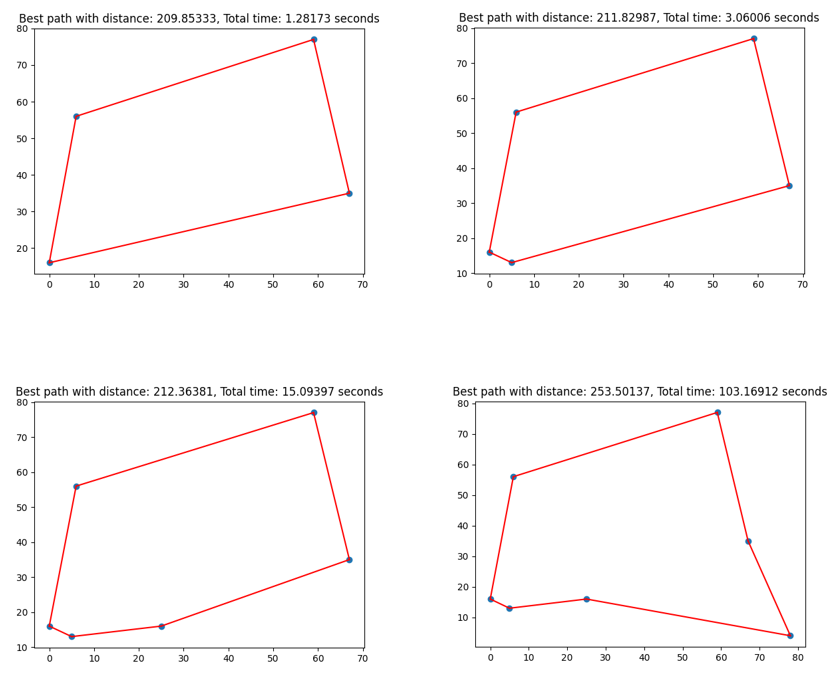
\includegraphics[width=0.8\textwidth]{
        papers/varalg/images/teil2/02BruteforceMethode.png
    }
    \caption{Resultate von verschiedener Durchgänge mit steigender Anzahl von Städten}
    \label{fig:results_bruteforce}
\end{figure}

Auf dem Bild \ref{fig:resultsbruteforce} ist ersichtlich, dass mit 
jedem weiteren Knoten der Aufwand exponentiell steigt. Anders 
ausgedrückt, mit jeder weiteren Stadt gibt es mehr Varianten, die 
durchprobiert werden müssen. Die Anzahl der Möglichkeiten lässt sich 
mit der Formel

\begin{equation}
    (n-1)!
\end{equation}

berechnen, wobei \(n\) die Anzahl der Städte ist.

Die Berechnung der verschiedenen Kombinationen lässt sich mit folgender 
mathematischen Formel beschreiben:

\begin{equation}
    \label{eq:bruteforce_min_formula}
    L(\sigma) = \sum_{i=1}^{n-1} d(\sigma(i), \sigma(i+1)) + d(\sigma(n), \sigma(1))
\end{equation}

\begin{itemize}
    \item \( L(\sigma) \) repräsentiert die Gesamtlänge der Rundreise, die durch
          die Permutation \( \sigma \) der Städte definiert ist.
    \item \( \sigma \) ist eine Permutation der Städte \( \{1, 2, \ldots, n\} \),
          wobei jede \( \sigma \) unterschiedliche Reihenfolge der Städte darstellt.
    \item \( d(i, j) \) ist die Funktion, welche die Entfernung der Stadt \( i \) und
          Stadt \( j \) zurückgibt.
    \item \( L(\sigma) \) ist die Gesamtlänge der Rundreise \( \sigma \).
\end{itemize}

\subsection{Kurzes Beispiel Rechnung der Formel
\label{buch:paper:varalg:subsection:bruteforce_calculate}}
\rhead{Kurzes Beispiel Rechnung der Formel}
Um zu verdeutlichen, wie die Formel \ref{eq:bruteforce_min_formula}
angewendet wird, folgt hier ein Beispiel.

\begin{table}[h]
    \centering
    \begin{tabular}{|c|c|c|c|c|}
        \hline
          & A  & B  & C  & D  \\ \hline
        A & 0  & 10 & 15 & 20 \\ \hline
        B & 10 & 0  & 35 & 25 \\ \hline
        C & 15 & 35 & 0  & 30 \\ \hline
        D & 20 & 25 & 30 & 0  \\ \hline
    \end{tabular}
    \caption{Beispiel Tabele mit möglicher Distanz der Städten}
    \label{tab:example_bruteforce_cities}
\end{table}

In der Tabelle \ref{tab:example_bruteforce_cities} sind die Distanzen 
zwischen den Städten A, B, C und D aufgeführt. Die Tabelle ist symmetrisch, 
da die Entfernung von Stadt A nach Stadt B gleich der Entfernung von 
Stadt B nach Stadt A ist.
Die Tabelle liesst sich wie folgt: Die Distanz zwischen Stadt B und D 25 beträgt.

Eine mögliche Permutation wäre $\sigma = (A, B, C, D)$ oder $\sigma = (B, D, A, C)$.

Setzt man die Permutation $\sigma = (B, D, A, C)$ in die Formel $\L(\sigma)$
\ref{eq:bruteforce_min_formula} ein, wird die Gesamtdistanz berechnet.


\(i\) und \(i+1\) definiert, welche Position in der Permutation betrachtet wird. 
Beispeil mit \( L(\sigma(1)) \) würde aus dem Set das B genommen und das führt 
dann zu dieser aufstellung
\begin{equation}
    L_1 = d(B, D) + d(D, A) + d(A, C) + d(C, B)
    = 25 + 20 + 15 + 35 = 95
\end{equation}
Dann werden alle möglichen Kombinationen durchgerechnet, und die kürzeste 
Strecke wird als Lösung gewählt.

\subsection{Aufwand Bruteforce
\label{buch:paper:varalg:subsection:bruteforce_efforts}}
\rhead{Aufwand Bruteforce}
Aus den vorherigen Abschnitten ist ersichtlich, dass der Aufwand für die 
Berechnung der kürzesten Strecke exponentiell steigt. Mit jedem weiteren 
Knoten gibt es mehr Variationen, die durchprobiert werden müssen. 
% Graph
\begin{figure}[h]
    \centering
    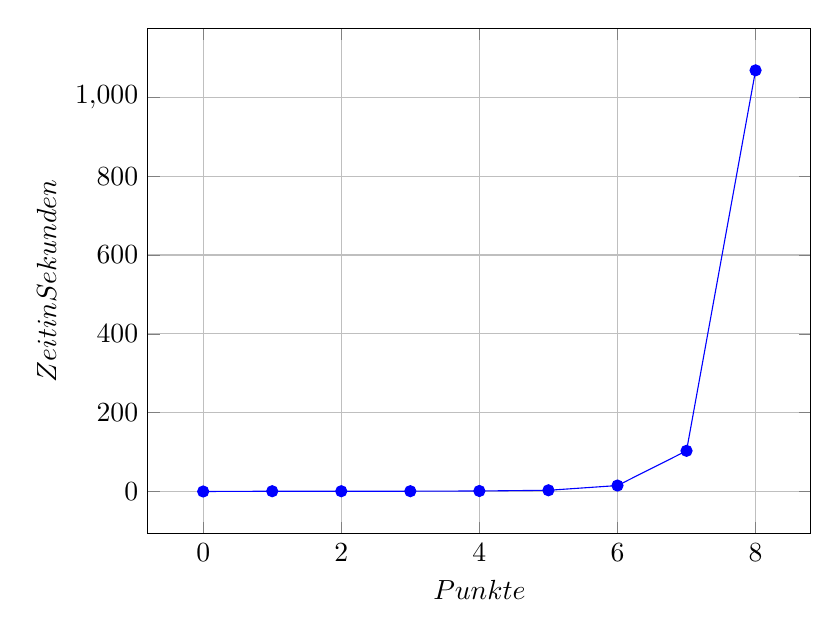
\begin{tikzpicture}
        \begin{axis}[
            xlabel=$Punkte$,
            ylabel=$Zeit in Sekunden$,
            grid=major,
            width=10cm,
            height=8cm
        ]
        \addplot[
            color=blue,
            mark=*
        ] coordinates {
            (0,0)
            (1,0.6880)
            (2,0.6905)
            (3,0.7666)
            (4,1.2817)
            (5,3.0601)
            (6,15.0940)
            (7,103.1691)
            (8,1068.3832)
        };
        \end{axis}
    \end{tikzpicture}
    \caption{Der Graph zeigt den Zeitverlauf mit steigender Anzahl von Städten}
    \label{fig:bruteforce_graph_time}
\end{figure}

% Tabelle
\begin{table}[ht]
    \centering
    \caption{Zeitverlauf mit steigender Anzahl von Städten}
    \begin{tabular}{cc}
        \toprule
        Punkte & Zeit in Sekunden      \\
        \midrule
        1      & 0.6880     \\
        2      & 0.6905     \\
        3      & 0.7666     \\
        4      & 1.2817     \\
        5      & 3.0601     \\
        6      & 15.0940    \\
        7      & 103.1691   \\
        8      & 1'068.3832 \\
        \bottomrule
    \end{tabular}
\end{table}

Aus der Tabelle und dem Graphen ist ersichtlich, dass der Aufwand mit 
jeder weiteren Stadt exponentiell steigt. Mit 8 Städten dauert die
Berechnung bereits über 17 Minuten.
